\PassOptionsToPackage{dvipsnames}{xcolor}
\documentclass[border=0mm]{standalone}
\usepackage{pgfplots}
\usepgfplotslibrary{groupplots}
\pgfplotsset{compat=1.17}
\usepackage[dvipsnames]{xcolor}
\usepackage{amsmath}
\usepackage{amssymb}
\usepackage{bm}


\begin{document}
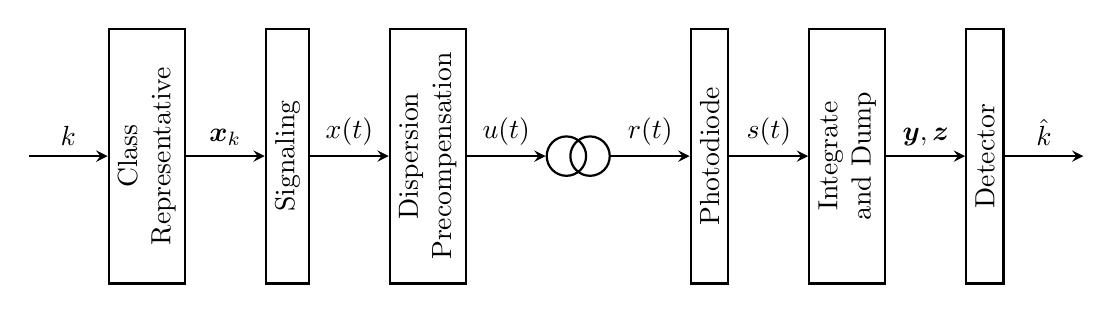
\begin{tikzpicture}[>=stealth,thick]%
\node [rectangle, draw, text width = 3cm, align = center, rotate=90,anchor=north] (CR) at (0,0) {Class\\Representative};
\node [rectangle, draw, text width = 3cm, align = center, rotate=90,anchor=north] (Sig) at($(CR.south)+(1,0)$) {Signaling};
\node [rectangle, draw, text width = 3cm, align = center, rotate=90,anchor=north] (DP) at($(Sig.south)+(1,0)$) {Dispersion\\Precompensation};
\node [circle, minimum width = 0.5cm, draw, rotate=90,anchor=north] (circ1) at($(DP.south)+(1,0)$) {};
\node [circle, minimum width = 0.5cm, draw, rotate=90,anchor=north] (circ2) at($(DP.south)+(1.3,0)$) {};
\node [rectangle, draw, text width = 3cm, align = center, rotate=90,anchor=north] (PD) at($(circ2.south)+(1,0)$) {Photodiode};
\node [rectangle, draw, text width = 3cm, align = center, rotate=90,anchor=north] (ID) at($(PD.south)+(1,0)$) {Integrate\\and Dump};
\node [rectangle, draw, text width = 3cm, align = center, rotate=90,anchor=north] (Det) at($(ID.south)+(1,0)$) {Detector};

\draw [->] (-1,0) -- node [above] {$k$}(CR); 
\draw [->] (CR.south) -- node [above] {$\bm x_k$} (Sig); 
\draw [->] (Sig.south) --  node [above] {$x(t)$} (DP); 
\draw [->] (DP.south) --  node [above] {$u(t)$} (circ1); 
\draw [->] (circ2.south) --  node [above] {$r(t)$} (PD); 
\draw [->] (PD.south) --  node [above] {$s(t)$} (ID); 
\draw [->] (ID.south) --  node [above] {$\bm y,\bm z$}(Det); 
\draw [->] (Det.south) -- node [above] {$\hat{k}$}+ (1,0);



\end{tikzpicture}

\end{document}
























